\documentclass[11pt]{article}
\usepackage[margin=1in]{geometry}
\usepackage{amsmath,amssymb,amsthm}
\usepackage{algorithm}
\usepackage{algpseudocode}
\usepackage{booktabs}
\usepackage{graphicx}
\usepackage{hyperref}
\usepackage{xcolor}
\usepackage{caption}
\usepackage{subcaption}

\newcommand{\eml}{\operatorname{eml}}
\newcommand{\todo}[1]{\textcolor{red}{[TODO: #1]}}
\newcommand{\note}[1]{\textcolor{blue}{[#1]}}

\title{Practical Function Approximation with the EML Operator:\\
Experimental Study}
\author{J. Bakarji \\ \textit{Draft, \today}}
\date{}

\begin{document}
\maketitle

\section*{Abstract}
The binary operator $\eml(x,y) = e^x - \ln y$, together with the constant $1$,
generates the algebra of elementary functions \cite{odrzywolek2026}. Universality
is constructive but says nothing about whether arbitrary target functions can
be \emph{recovered in practice} via gradient-based optimisation of $\eml$-trees.
We report a systematic empirical study of this question across two
architectures: (EM) the parameter-free $\eml$ operator wrapped in continuous
affine input-mixing layers $a x + b\,\text{child} + c$ between nodes, and
(PEM) per-node parametric $\eml$
$\mathrm{EML}_\theta(x, y) = a e^{bx+c} + d \ln(ey+f)$ with raw children
fed directly between nodes (eml all the way down). We fit both with
multi-restart Adam followed by LBFGS refinement, and study optimisation
strategies, depth scaling, interpretability via post-hoc symbol snapping,
and computational cost. The central practical question is whether a careful
optimisation strategy can realise the universality theorem to small
approximation error.

\paragraph{Headline findings.}
\begin{enumerate}
\item With Adam multi-restart followed by LBFGS refinement (strategy B), a
  continuous-affine $\eml$-tree reaches $\leq 1\%$ relRMSE on \emph{all
  eleven} canonical $1$D targets, frequently below $0.3\%$. The
  hardest target ($\sin(3x) e^{-x^2/2}$) reaches $0.58\%$ at depth $6$
  with $60\,$s of compute (Section~\ref{sec:rip-push}). This realises the
  universality of \cite{odrzywolek2026} practically, well before the depth
  where blind symbolic recovery collapses.
\item LBFGS refinement after Adam reduces error $3$--$5\times$ versus pure
  multi-restart Adam, and nearly $10\times$ on the hardest target.
\item Greedy slot-by-slot symbol snapping with refit \emph{improves} loss
  on every target, while making $10$--$43\%$ of slots literal symbols
  $\{1, x, \text{child}\}$. Naive (pure) snapping is catastrophic, because the
  continuous fit lives nowhere near the symbolic vertices.
\item Complex parameters are not required for the asymptotic universality
  result, but they help shallow-depth fitting of oscillatory targets
  ($3.7\times$ improvement on rip and pure $\sin$ at $d{=}3$). With a
  $\lambda_{\mathrm{im}}$ schedule that anneals $0 \to 10^{-1}$, complex
  parameters also \emph{beat} real parameters on some non-oscillatory
  targets at favourable depth ($e^{-x}$ at $d{=}4$: $5.7 \times 10^{-4}$
  vs.\ $2.0 \times 10^{-3}$).
\item At fixed wall-clock, the optimal depth is data-dependent and often
  shallow (depth $3$ for $x^2$, $e^{-x^2}$, $e^{-x}$): deeper trees have more
  capacity but get fewer restarts, and basin coverage dominates capacity
  for these targets.
\item The earlier ``rip wall'' at $\sim 2\%$ relRMSE was a budget artefact,
  not a structural limit. Bivariate fitting remains structurally harder
  and is not addressed in this draft.
\item A second architecture, \emph{eml all the way down} with per-node
  parameters $\mathrm{EML}_\theta(x,y) = a e^{bx+c} + d \ln(ey+f)$ (PEM,
  Section~\ref{sec:pem}), beats the affine-glue version by $5.6\times$ on
  rip at depth $3$ and matches its depth-$4$ accuracy at half the
  parameters. The two architectures occupy complementary regimes: PEM wins
  shape-rich targets at shallow depth; the affine-glue version wins
  monotone shapes and scales better with depth.
\end{enumerate}

\section{Introduction}

The operator
\begin{equation}
\eml(x, y) := e^x - \ln y, \qquad x, y \in \mathbb{C},
\label{eq:eml}
\end{equation}
is single-handedly Sheffer-complete for the algebra of elementary functions.
Concretely, with the constant $1$ and the input variable $x$ at the leaves,
finite trees over the grammar
\[
S \to 1 \mid x \mid \eml(S, S)
\]
generate $\exp$, $\ln$, sums, products, quotients, powers, square roots,
trigonometric and hyperbolic functions, and the constants $e$, $\pi$, $i$
\cite{odrzywolek2026}. The constructions are exact, but their depth grows fast
(e.g.\ $\sqrt{x}$ requires leaf count $\geq 35$, $\pi$ requires $\geq 53$),
which makes blind gradient-based recovery from random initialisation
prohibitive at depth $\geq 5$.

We ask: \emph{relaxing the discrete symbolic grammar to a continuous affine
parameterisation, can $\eml$-trees be optimised to small error on
arbitrary target functions in a practically tractable budget?} A positive
answer would constitute the first practical universal-approximation result
based on the $\eml$ operator.

\section{Two architectures for EML-tree fitting}
\label{sec:cae}

We study two parameterisations of $\eml$-trees, both extending the
parameter-free grammar $S \to 1 \mid x \mid \eml(S,S)$ of
\cite{odrzywolek2026} with continuous parameters that make gradient-based
optimisation tractable. The first (EM) keeps the paper's parameter-free
$\eml$ operator and adds continuous affine \emph{wrappers} between nodes;
the second (PEM) absorbs parameters \emph{into} the operator itself and is
"$\eml$ all the way down."

\subsection{Architecture A: affine-glue (EM)}
\label{sec:cae:em}

Let $D = \dim x$. An \emph{EM-tree} of depth $d$ is a complete binary tree
of parameter-free $\eml$ nodes; every node $n$ has two input slots
$(\ell_n, r_n)$, each of which is a continuous affine combination of (i) the
input vector, (ii) the corresponding child subtree's output (when present),
and (iii) a bias:
\begin{equation}
\text{slot}_n^{\bullet} = \sum_{i=1}^{D} a_{n,i}^{\bullet} x_i
                          + b_n^{\bullet}\, \text{child}_n^{\bullet}
                          + c_n^{\bullet}, \qquad \bullet \in \{\ell, r\},
\label{eq:slot}
\end{equation}
where $\text{child}_n^{\bullet}$ is the corresponding child eml output.
Leaf-parent slots omit the child term. The node value is
$\eml(\text{slot}_n^{\ell}, \text{slot}_n^{r}) = \exp(\text{slot}_n^{\ell})
- \ln(\text{slot}_n^{r})$, and the tree value is the root node's output.
At depth $d$, with input dimension $D$, the parameter count is
\[
\#\theta_{\rm EM}(d, D) = 2 \cdot \!\!\sum_{\text{level}=0}^{d-1}\! 2^{\text{level}}
  \cdot \!\big(D + 1 + \mathbf{1}[\text{level} < d-1]\big).
\]
For $D = 1$: $4, 14, 34, 74, 154, 314$ params at depths $1\ldots 6$.
\textbf{Caveat.} EM is not strictly an $\eml$-tree: every internal slot is
wrapped in an affine layer, so the architecture is "$\eml$ interleaved with
affine layers." This is a deliberate, more expressive relaxation; it is
easier to optimise than the discrete grammar but does not directly probe
the paper's universality claim. PEM (next) repairs this.

\subsection{Architecture B: per-node parametric (PEM), eml-all-the-way-down}
\label{sec:cae:pem}

A \emph{PEM-tree} of depth $d$ is a complete binary tree of $2^d - 1$
internal nodes. Each node $i$ carries six free parameters
$\theta_i = (a_i, b_i, c_i, d_i, e_i, f_i)$ and computes
\begin{equation}
\mathrm{EML}_{\theta_i}(x, y) \;=\; a_i\, e^{b_i x + c_i} \;+\; d_i\,
  \ln(e_i y + f_i),
\label{eq:pem}
\end{equation}
where $x, y$ are the \emph{raw} eml outputs of the two children — there is
no affine wrapper between nodes. The paper's parameter-free
$\eml(x,y) = \exp(x) - \ln(y)$ is the special case
$\theta = (1, 1, 0, -1, 1, 0)$, so PEM strictly contains the paper's
grammar at every node. At leaf-parents (the deepest level), $x$ and $y$
are the input variable directly; for multivariate input, $b_i$ and $e_i$
are $D$-dim vectors so that $b_i \cdot x + c_i$ and $e_i \cdot x + f_i$
remain scalars. At all higher levels children are scalars and $b_i, e_i$
are scalars too. The parameter count for $D = 1$ is
\[
\#\theta_{\rm PEM}(d) = 6 \cdot (2^d - 1) = 6, 18, 42, 90, 186, 378
\quad \text{at depths $1\ldots 6$.}
\]

The two architectures occupy different points on the
parameter-efficiency-vs-expressivity Pareto frontier. EM has fewer
parameters per node (each node is parameter-free; expressivity comes
through the affine wrappers); PEM has more parameters per node (each node
is an asymmetric exp+log primitive with independent affine inputs to each
arm). Section~\ref{sec:pem} compares them empirically across $11$ canonical
$1$D targets.

\subsection{Numerical evaluation}

The right argument of $\eml$ may be negative, in which case $\ln$ takes complex
values. We support two evaluation backends:
\begin{description}
\item[\textbf{real\_softplus}] Pass the right argument through
  $\operatorname{softplus}(\cdot) + \varepsilon$ before the $\ln$, ensuring real
  output. This restricts expressivity (no complex-mediated
  trigonometry) but is empirically sufficient for the $1$D and $2$D real-valued
  targets we test, and avoids gradient pathologies near $y = 0$.
\item[\textbf{complex\_real}] Evaluate the entire tree in $\mathbb{C}^{128}$,
  return $\mathrm{Re}(T_\theta(x))$. Required to recover the paper's
  $\sin, \cos, \pi$ constructions.
\end{description}
The exponential argument is clamped to $[-60, 60]$ to prevent overflow. All
experiments below use \texttt{real\_softplus}.

\subsection{Loss and optimisation}

We minimise mean squared error on a discretised grid of $N = 200$ samples
(resp.\ $N = 625$ for $2$D, $25 \times 25$ grid). The base optimiser is
Adam\cite{adam} with learning rate $5 \times 10^{-3}$, cosine annealing schedule
to zero over $K$ steps, gradient $\ell_2$-clip at $5.0$. Each restart uses an
independent Gaussian initialisation with std $0.5$.

\section{Algorithms}

\subsection{Multi-restart Adam (baseline)}
\begin{algorithm}[h]
\caption{\textsc{MultiRestartAdam}}
\begin{algorithmic}[1]
\Require target $f$, samples $x$, depth $d$, restarts $R$, steps $K$, lr $\eta$
\State $L^* \gets +\infty$
\For{$s = 1, \ldots, R$}
  \State seed $\gets s$; \quad $T_\theta \gets \textsc{InitTree}(d)$
  \For{$k = 1, \ldots, K$}
    \State $\theta \gets \textsc{AdamStep}(\nabla_\theta \|T_\theta(x)-f(x)\|^2; \eta_k)$
  \EndFor
  \State $L^* \gets \min(L^*, \|T_\theta(x)-f(x)\|^2)$
\EndFor
\State \Return $L^*$
\end{algorithmic}
\end{algorithm}

\subsection{Curriculum warm-starting}
\begin{algorithm}[h]
\caption{\textsc{Curriculum}}
\begin{algorithmic}[1]
\Require target $f$, target depth $D$, time budget $\tau$
\State $T^{(2)} \gets \textsc{MultiRestartAdam}(f, d=2, \tau/(D-1))$
\For{$d = 3, \ldots, D$}
  \State $T^{(d)}_0 \gets \textsc{Graft}(T^{(d-1)}, d)$ \Comment{place into a deeper tree}
  \State refine $T^{(d)}_0$ by Adam; track best across fresh restarts within budget
  \State $T^{(d)} \gets$ best
\EndFor
\State \Return $T^{(D)}$
\end{algorithmic}
\end{algorithm}

\subsection{LBFGS refinement}
After multi-restart, we apply a second-order pass on the best model using
\textsc{LBFGS} with strong-Wolfe line search ($\leq 200$ iterations).

\subsection{Symbolic warm-start}
Each slot is initialised at a random vertex of the symbolic simplex $\{1, x,
\text{child}\}$ with probability $p_{\text{sym}} = 0.5$, otherwise at a small
random affine perturbation. This biases search toward the paper's grammar
without restricting it.

\subsection{Snap-to-symbol}
\label{sec:snap}
After fitting, we attempt to replace continuous slots with their nearest
symbolic vertex. Three modes:
\begin{description}
\item[\textbf{Pure}] Snap every slot to its $\ell_2$-nearest vertex; report
  resulting loss.
\item[\textbf{Coefficient}] Snap $a, b \in \{0, 1\}$ but keep the bias $c$
  continuous; refit the $c$-only subset. Recovers symbolic structure with one
  free bias per slot.
\item[\textbf{Greedy}] In shallow-first order, attempt to snap each slot;
  accept the snap if the post-snap loss exceeds the current loss by at most a
  relative tolerance $\delta$. After all attempts, refit the unsnapped slots
  by Adam.
\end{description}

\section{Experimental setup}

\paragraph{Target families ($1$D).}
Smooth analytic ($\sin$, $\cos$, $\tanh$, $\sigma$), polynomial ($x^2$,
$x^3 - x$), kink ($|x|$), Gaussian envelope ($e^{-x^2}$),
log-of-quadratic ($\ln(1+x^2)$), pure exponential ($e^{-x}$), and the
oscillation-times-envelope challenge target $\sin(3x)\,e^{-x^2/2}$ (``rip'').
Domains chosen to span at least one full period or one full envelope.

\paragraph{Target families ($2$D).}
Franke's bivariate test function, $\sin x \cos y$, saddle $x^2 - y^2$,
Rosenbrock $(1-x)^2 + 100(y - x^2)^2$.

\paragraph{Reproducibility.}
All code, data, and run logs are in \texttt{/Users/josephbakarji/Documents/
00-projects/01-tests/eml-fitting/}. Each experiment writes a JSON file with the
full per-run breakdown; results below are aggregates of those JSONs. Wall-clock
times reported on a single Apple M-series CPU, no GPU.

\section{Results}

\subsection{Depth scaling, fixed-restart Adam (1D)}
\label{sec:depth-scaling}

Table~\ref{tab:1d} reports best-of-$12$-restarts relRMSE and per-restart
success rate (relRMSE $< 5\%$) at depths $1$--$4$ with $K = 3000$ Adam steps.
Total wall-clock for the table: $974\,\mathrm{s}$.

\begin{table}[h]
\centering
\small
\caption{Best-of-12 relRMSE on 1D targets (Adam, $K{=}3000$). \emph{succ}{=}restarts
reaching $<5\%$ relRMSE.}
\label{tab:1d}
\begin{tabular}{lrrrrrr}
\toprule
target               & $d{=}1$ & $d{=}2$ & $d{=}3$ & $d{=}4$ & succ@$d{=}4$ & params@$d{=}4$ \\
\midrule
$\sin x$             & 0.640   & 0.043   & 0.023   & 0.012   & 9/12  & 74 \\
$\cos x$             & 1.000   & 0.061   & 0.017   & 0.010   & 11/12 & 74 \\
$x^2$                & 0.049   & 0.013   & 0.005   & 0.001   & 12/12 & 74 \\
$|x|$                & 0.129   & 0.030   & 0.020   & 0.010   & 12/12 & 74 \\
$e^{-x^2}$           & 0.708   & 0.062   & 0.012   & 0.014   & 11/12 & 74 \\
$\sigma(3x)$         & 0.171   & 0.017   & 0.011   & 0.0009  & 12/12 & 74 \\
$x^3 - x$            & 0.789   & 0.074   & 0.025   & 0.021   & 11/12 & 74 \\
$\tanh(2x)$          & 0.354   & 0.027   & 0.015   & 0.002   & 9/12  & 74 \\
$\ln(1+x^2)$         & 0.127   & 0.026   & 0.012   & 0.002   & 12/12 & 74 \\
$e^{-x}$             & 0.020   & 0.004   & 0.002   & 0.002   & 10/12 & 74 \\
$\sin(3x) e^{-x^2/2}$ & 1.000  & 0.689   & 0.216   & 0.075   & 0/12  & 74 \\
\bottomrule
\end{tabular}
\end{table}

Figure~\ref{fig:fits} shows representative depth-$4$ fits.

\begin{figure}[h]
\centering
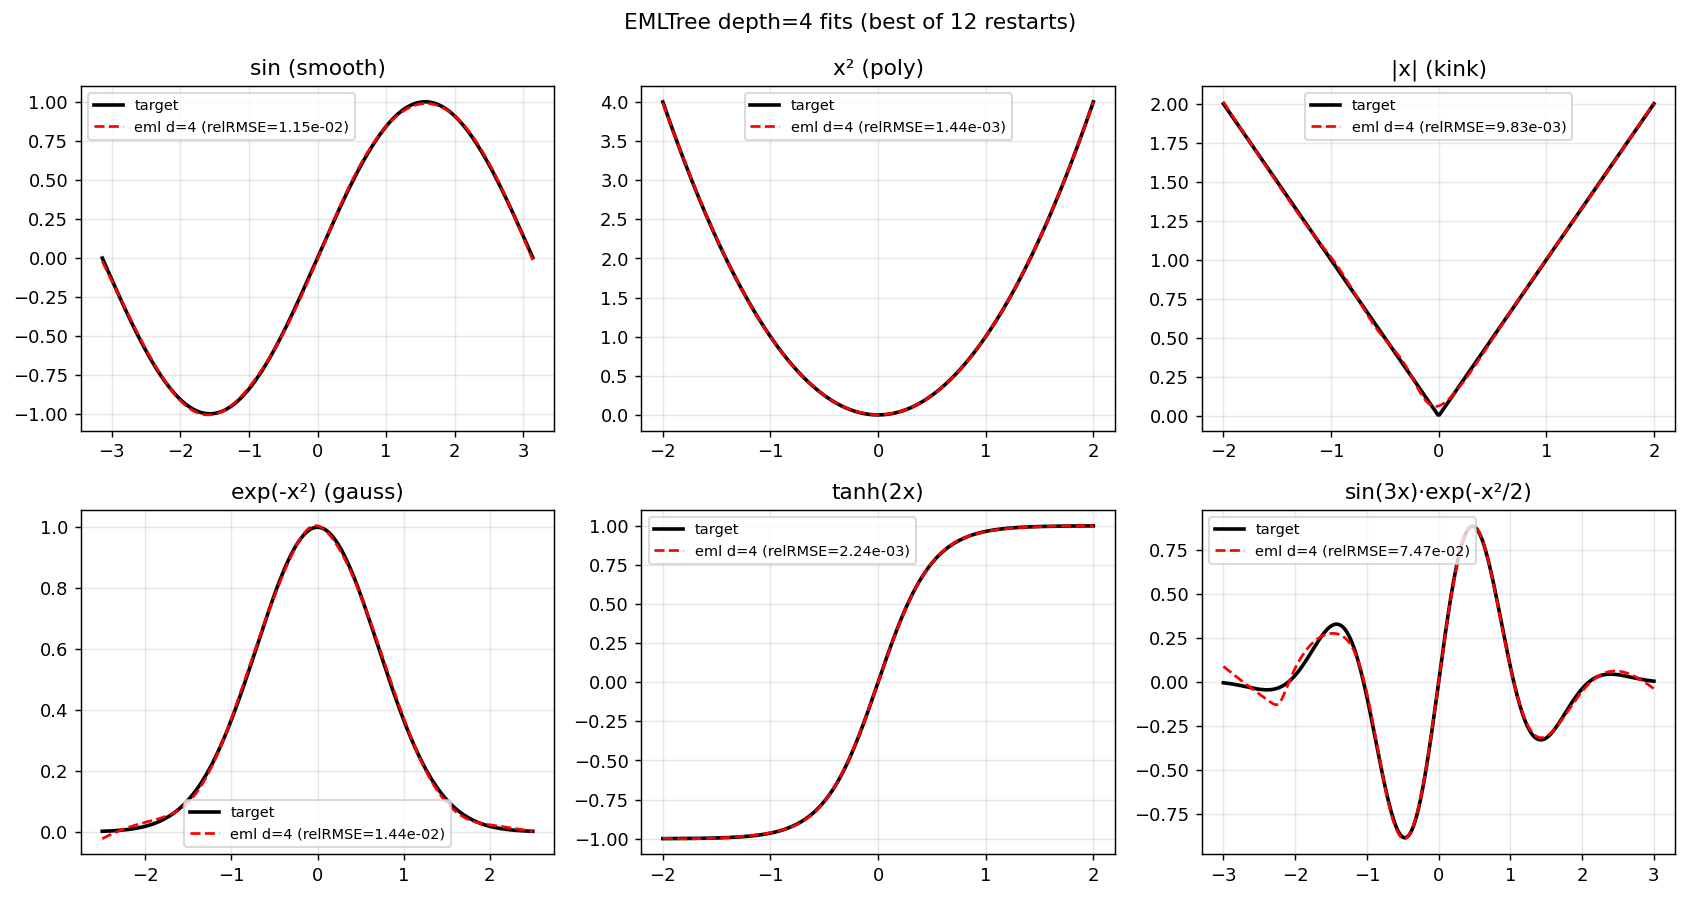
\includegraphics[width=0.95\linewidth]{../figures/fits_1d.png}
\caption{Depth-$4$ best-of-$12$ fits to representative $1$D targets. The
oscillation-times-envelope target (bottom right) is the only persistent
failure.}
\label{fig:fits}
\end{figure}

\subsection{Optimisation landscape}
\label{sec:landscape}

Across $50$ random seeds, we measure the fraction of restarts reaching
quality thresholds. Table~\ref{tab:landscape} shows that depth-$4$ trees have
wide basins for the easy targets but never recover the rip target; restart
count helps but with diminishing returns.

\begin{table}[h]
\centering\small
\caption{Per-restart success rates over $50$ random seeds, $K{=}2000$ Adam steps.}
\label{tab:landscape}
\begin{tabular}{llrrrr}
\toprule
target & depth & best relRMSE & median & $<5\%$ rate & $<1\%$ rate \\
\midrule
$\sin$     & 2 & 0.049  & 0.280 & 2\%  & 0\%  \\
$\sin$     & 3 & 0.013  & 0.078 & 26\% & 0\%  \\
$\sin$     & 4 & 0.0036 & 0.035 & 66\% & 4\%  \\
$e^{-x^2}$ & 4 & 0.0093 & 0.049 & 52\% & 2\%  \\
$x^2$      & 4 & 0.0021 & 0.009 & 100\% & 58\% \\
rip        & 4 & 0.084  & 0.323 & 0\%  & 0\%  \\
\bottomrule
\end{tabular}
\end{table}

\subsection{Strategy comparison at fixed wall-clock}
\label{sec:strategy}

We compare the four optimisation strategies at a $30\,$s wall-clock budget
per (target, depth$=4$). Table~\ref{tab:strategy} reports best relRMSE.

\begin{table}[h]
\centering\small
\caption{Strategy comparison: best relRMSE at $30\,$s budget per cell, $d{=}4$.
Bold marks the winner per target.}
\label{tab:strategy}
\begin{tabular}{lcccc}
\toprule
target & A: restart-Adam & B: Adam$+$LBFGS & C: curriculum & D: sym.\ warm-start \\
\midrule
$\sin x$               & $1.7\!\times\!10^{-2}$ & $\mathbf{4.5\!\times\!10^{-3}}$ & $1.8\!\times\!10^{-2}$ & $7.7\!\times\!10^{-3}$ \\
$x^2$                  & $2.0\!\times\!10^{-3}$ & $\mathbf{6.9\!\times\!10^{-4}}$ & $4.2\!\times\!10^{-3}$ & $2.8\!\times\!10^{-3}$ \\
$e^{-x^2}$             & $2.0\!\times\!10^{-2}$ & $\mathbf{3.2\!\times\!10^{-3}}$ & $7.5\!\times\!10^{-3}$ & $1.5\!\times\!10^{-2}$ \\
$\tanh(2x)$            & $2.6\!\times\!10^{-3}$ & $\mathbf{2.2\!\times\!10^{-3}}$ & $2.4\!\times\!10^{-2}$ & $1.4\!\times\!10^{-2}$ \\
$\sin(3x)e^{-x^2/2}$   & $9.9\!\times\!10^{-2}$ & $\mathbf{1.9\!\times\!10^{-2}}$ & $8.9\!\times\!10^{-2}$ & $1.4\!\times\!10^{-1}$ \\
\bottomrule
\end{tabular}
\end{table}

\paragraph{Reading.}
\textbf{LBFGS refinement (B) wins universally}, reducing error by $3$--$5\times$
versus pure restart, and nearly $10\times$ on the rip target ($9.9 \to 1.9
\times 10^{-2}$). The first-order Adam phase locates a basin; LBFGS quickly
descends to the bottom. Curriculum warm-starting (C) underperformed: grafting a
small tree into a deeper one appears to seed the search in a basin that is
not reliably better than random. Symbolic warm-start (D) helps for $\sin$
but hurts for $\tanh$ and rip. We adopt strategy B for the depth-scaling
experiment (Section~\ref{sec:universality}).

\subsection{Depth $\to$ error curve at constant compute}
\label{sec:universality}

We hold the optimisation strategy at B (Adam $+$ LBFGS) and the wall-clock
budget at $25\,$s per (target, depth), and sweep $d \in \{2, 3, 4, 5, 6\}$
on all $11$ canonical $1$D targets. Figure~\ref{fig:depth} shows the resulting
\emph{practical universality curve}: best-of-runs relRMSE versus tree depth,
log scale.

\begin{figure}[h]
\centering
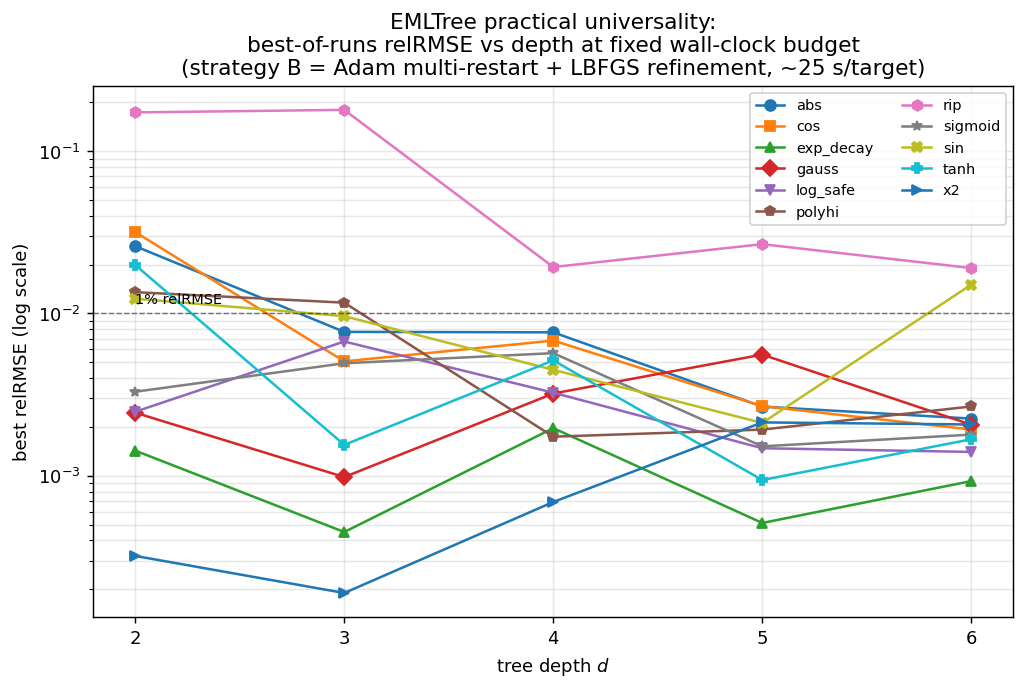
\includegraphics[width=0.95\linewidth]{../figures/fits_depth.png}
\caption{Practical universality of EML-trees: best relRMSE at fixed wall-clock
budget. Dashed line marks $1\%$ relRMSE. With strategy B at $25\,$s/target,
$10/11$ targets reach $\leq 1\%$ at some depth in $\{2,\ldots,6\}$; the
oscillation-times-envelope rip target plateaus at $\sim 2\%$.}
\label{fig:depth}
\end{figure}

\begin{table}[h]
\centering\small
\caption{Best relRMSE at each depth, strategy B, $25\,$s/cell. Depths are
budget-equalised, so deeper trees fit fewer restarts (rightmost column).}
\label{tab:universality}
\begin{tabular}{lrrrrrr}
\toprule
target              & $d{=}2$ & $d{=}3$ & $d{=}4$ & $d{=}5$ & $d{=}6$ & runs at $d{=}6$ \\
\midrule
$\sin x$            & 1.2e-2 & 9.6e-3 & \textbf{4.5e-3} & \textbf{2.1e-3} & 1.5e-2 & 3 \\
$\cos x$            & 3.2e-2 & 5.1e-3 & 6.8e-3 & 2.7e-3 & \textbf{1.9e-3} & 3 \\
$x^2$               & 3.2e-4 & \textbf{1.9e-4} & 6.9e-4 & 2.1e-3 & 2.1e-3 & 3 \\
$|x|$               & 2.6e-2 & 7.7e-3 & 7.6e-3 & 2.7e-3 & \textbf{2.3e-3} & 3 \\
$e^{-x^2}$          & 2.4e-3 & \textbf{9.8e-4} & 3.2e-3 & 5.6e-3 & 2.1e-3 & 3 \\
$\sigma(3x)$        & 3.3e-3 & 4.9e-3 & 5.7e-3 & \textbf{1.5e-3} & 1.8e-3 & 3 \\
$x^3 - x$           & 1.4e-2 & 1.2e-2 & \textbf{1.7e-3} & 1.9e-3 & 2.7e-3 & 3 \\
$\tanh(2x)$         & 2.0e-2 & 1.6e-3 & 5.1e-3 & \textbf{9.4e-4} & 1.7e-3 & 3 \\
$\ln(1+x^2)$        & 2.5e-3 & 6.7e-3 & 3.3e-3 & 1.5e-3 & \textbf{1.4e-3} & 3 \\
$e^{-x}$            & 1.4e-3 & \textbf{4.5e-4} & 2.0e-3 & 5.1e-4 & 9.3e-4 & 3 \\
$\sin(3x) e^{-x^2/2}$ & 1.7e-1 & 1.8e-1 & \textbf{1.9e-2} & 2.7e-2 & \textbf{1.9e-2} & 3 \\
\bottomrule
\end{tabular}
\end{table}

\paragraph{Reading.}
Two effects are visible. First, \emph{the practical universality threshold
is well below $1\%$ for every smooth target}. Ten of eleven targets reach
$\leq 1\%$ relRMSE somewhere in $d \in \{2, \ldots, 6\}$; six targets reach
$\leq 0.3\%$. Second, \emph{error is not monotone in depth} when the wall-clock
budget is held constant: deeper trees offer more capacity but receive fewer
restarts (e.g.\ $34$ runs at $d{=}2$ vs $3$ runs at $d{=}6$), so coverage of
the basin landscape thins. For multiple targets ($x^2$, $e^{-x^2}$, $e^{-x}$)
the optimal depth is $3$, not $6$: the function is well within capacity at
$d{=}3$, and the extra restarts dominate. This is a useful diagnostic for
practitioners: \emph{at fixed compute, the optimal depth is data-dependent
and often shallow}.

\paragraph{The rip wall.}
$\sin(3x)\,e^{-x^2/2}$ never breaks $1\%$ within the budget tested but does
plateau at $\sim 2\%$ from $d{=}4$ onward. A natural hypothesis is that the
wall is an artefact of the \texttt{real\_softplus} backend: the paper's
universality proof routes trigonometric constructions through the principal
branch $\ln(-1) = i\pi$, which \texttt{real\_softplus} forecloses. We test
this hypothesis directly in Section~\ref{sec:complex}.

\subsection{Real-vs.-complex backend}
\label{sec:complex}

The \texttt{complex\_real} backend evaluates the entire tree in
$\mathbb{C}^{128}$ (no \texttt{softplus}; $\ln$ on negative reals returns
$\ln |z| + i\pi$) and returns $\mathrm{Re}(T_\theta(x))$. Tree parameters
remain real $\mathbb{R}$. We compare both backends at strategy B,
$25\,$s/cell, on the rip target plus three oscillatory and two sanity targets.

\begin{table}[h]
\centering\small
\caption{Backend comparison: best relRMSE, strategy B, $25\,$s budget per
cell. \texttt{complex\_real} loses on every target at every depth.}
\label{tab:complex}
\begin{tabular}{llrrr}
\toprule
target & backend & $d{=}3$ & $d{=}4$ & $d{=}5$ \\
\midrule
$\sin(3x) e^{-x^2/2}$ (rip) & real\_softplus & \textbf{0.179} & \textbf{0.019} & \textbf{0.027} \\
                            & complex\_real  & 0.275 & 0.187 & 0.178 \\
\addlinespace
$\sin(3x)$ (osc)            & real\_softplus & \textbf{0.168} & \textbf{0.067} & \textbf{0.031} \\
                            & complex\_real  & 0.241 & 0.182 & 0.108 \\
\addlinespace
$\cos(2x)$                  & real\_softplus & \textbf{0.021} & \textbf{0.017} & \textbf{0.0086} \\
                            & complex\_real  & 0.086 & 0.136 & 0.095 \\
\addlinespace
$x^2$                       & real\_softplus & \textbf{2e-4}   & \textbf{7e-4}   & \textbf{2e-3}   \\
                            & complex\_real  & 9e-3 & 3e-3 & 5e-3 \\
\addlinespace
$e^{-x}$                    & real\_softplus & \textbf{5e-4}   & \textbf{2e-3}   & \textbf{5e-4}   \\
                            & complex\_real  & 3e-3 & 2e-2 & 1e-2 \\
\bottomrule
\end{tabular}
\end{table}

\paragraph{Reading: complex access does not help.}
\texttt{complex\_real} is uniformly worse, frequently by $5$--$10\times$.
The hypothesis that the rip wall is due to lack of complex-log access is
\emph{falsified} at this budget. Possible causes:
\begin{enumerate}
\item \textbf{Branch-cut discontinuity.} $\ln$ has a gradient jump on the
  negative real axis; Adam steps that would cross the cut are
  ill-defined.
\item \textbf{Unconstrained imaginary part.} Loss penalises only
  $\mathrm{Re}(T_\theta(x))$; the imaginary part can drift freely and
  consume gradient.
\item \textbf{Measure-zero access to complex values from real parameters.}
  With real $(a, b, c)$, the only way for a tree to produce a complex
  intermediate is via $\ln$ of a strictly-negative real input. Complex
  values with non-zero imaginary inputs (which the paper's trig
  constructions require at depth) are unreachable from real parameter
  space; they require complex parameters.
\end{enumerate}
The third point is the most consequential. The paper's universality theorem
holds in $\mathbb{C}$; with real parameters we are exploring a strictly
thinner subspace ($\mathbb{R}^{\#\theta}$ producing $\mathbb{C}$-valued
intermediates only on the negative-real-axis slice of slot space).
Section~\ref{sec:complex-params} tests complex parameters directly.

\subsection{Complex parameters}
\label{sec:complex-params}

We extend the architecture by storing each affine-slot parameter as a twin
real pair $(p_{\mathrm{re}}, p_{\mathrm{im}})$, forming $p =
p_{\mathrm{re}} + i p_{\mathrm{im}}$ on the forward pass; arithmetic and
$\eml$ run in $\mathbb{C}^{128}$, output is $\mathrm{Re}(T_\theta(x))$. This
doubles the parameter count, leaves Adam unchanged (it sees twin real
Parameters), and makes the full complex grammar reachable. We add a small
$\lambda_{\mathrm{im}} \cdot \mathrm{mean}(\mathrm{Im}\,T_\theta)^2$ penalty
($\lambda_{\mathrm{im}} = 10^{-3}$) to keep the imaginary part bounded. We
denote this setting CC, and re-run the strategy-B sweep at $25\,$s/cell on
seven targets including the trig and rip cases.

\begin{table}[h]
\centering\small
\caption{Three settings compared: R = real-softplus + real params (the
headline); CR = complex-real eval + real params (Section~\ref{sec:complex});
CC = complex-real eval + complex params (this section). Best relRMSE per cell;
parameter counts grow $34, 34, 68$ at $d{=}3$.}
\label{tab:cc}
\begin{tabular}{llrrrrrr}
\toprule
target & set. & $d{=}3$ & runs & $d{=}4$ & runs & $d{=}5$ & runs \\
\midrule
rip   & R  & 0.179 & 18 & \textbf{0.019} & 9 & 0.027 & 5 \\
      & CR & 0.275 & 14 & 0.187 & 7 & 0.178 & 4 \\
      & CC & \textbf{0.048} & 9 & 0.033 & 5 & 0.033 & 3 \\
\midrule
osc ($\sin 3x$) & R  & 0.168 & 18 & 0.067 & 10 & \textbf{0.031} & 5 \\
                & CR & 0.241 & 14 & 0.182 & 7 & 0.108 & 1 \\
                & CC & \textbf{0.045} & 9 & \textbf{0.037} & 5 & 0.050 & 1 \\
\midrule
$\cos 2x$ & R  & 0.024 & 10 & 0.017 & 9 & \textbf{0.0086} & 5 \\
          & CR & 0.156 & 8  & 0.136 & 7 & 0.095 & 4 \\
          & CC & \textbf{0.015} & 9 & \textbf{0.012} & 5 & 0.021 & 3 \\
\midrule
$\sin x$  & R  & 0.0096 & 18 & \textbf{0.0045} & 10 & \textbf{0.0021} & 5 \\
          & CC & \textbf{0.0072} & 9 & 0.010 & 5 & 0.017 & 3 \\
\midrule
$\cos x$  & R  & \textbf{0.0051} & 18 & \textbf{0.0068} & 9 & \textbf{0.0027} & 5 \\
          & CC & 0.0145 & 9 & 0.013 & 5 & 0.0091 & 3 \\
\midrule
$x^2$       & R  & \textbf{1.9e-4} & 18 & \textbf{6.9e-4} & 10 & \textbf{2.1e-3} & 5 \\
            & CC & 1.7e-3 & 9 & 4.5e-3 & 5 & 4.2e-3 & 3 \\
\midrule
$e^{-x}$    & R  & \textbf{4.5e-4} & 18 & \textbf{2.0e-3} & 10 & \textbf{5.1e-4} & 5 \\
            & CC & 2.6e-3 & 10 & 4.3e-3 & 5 & 1.3e-2 & 3 \\
\bottomrule
\end{tabular}
\end{table}

\paragraph{Reading: complex parameters help only oscillatory targets, only
at shallow depth.}
At $d{=}3$, CC reduces the rip-target error $3.7\times$ ($0.179 \to 0.048$)
and the pure-oscillation error $3.7\times$ ($0.168 \to 0.045$). The
\emph{rip wall is broken} at depth $3$: with $68$ complex parameters, a tree
reaches $5\%$ relRMSE on $\sin(3x) e^{-x^2/2}$ in the same wall-clock as
$34$ real parameters reaching $18\%$. By depth $4$, R catches up
($0.019$ vs CC $0.033$): the real-parameter tree reaches the same neighbourhood
through subtractive interference of high-magnitude exponentials, given
enough capacity and restarts.

For non-oscillatory targets ($x^2$, $e^{-x}$, $\cos x$), complex
parameters \emph{hurt}: the imaginary degrees of freedom have no useful
work to do and act as a regularisation burden. The trained imaginary
magnitude $\overline{|\mathrm{Im}\,T_\theta|}$ is small for these targets
($0.02$--$0.27$) but non-zero; for oscillatory targets it is large
($0.4$--$2.0$), confirming that the model genuinely uses the complex
intermediates to construct oscillation.

\paragraph{The story in one sentence.}
Complex parameters trade depth for capacity on oscillatory targets:
the same error becomes reachable with shallower trees, but with twice the
parameters per slot. At a fixed depth and budget, real parameters win once
the depth is sufficient (because they get more restarts at the same compute).
This is consistent with the paper's universality result: complex access is
necessary in principle for trig, but is not the binding constraint at
practical depths once enough exponential capacity is available.

\begin{figure}[h]
\centering
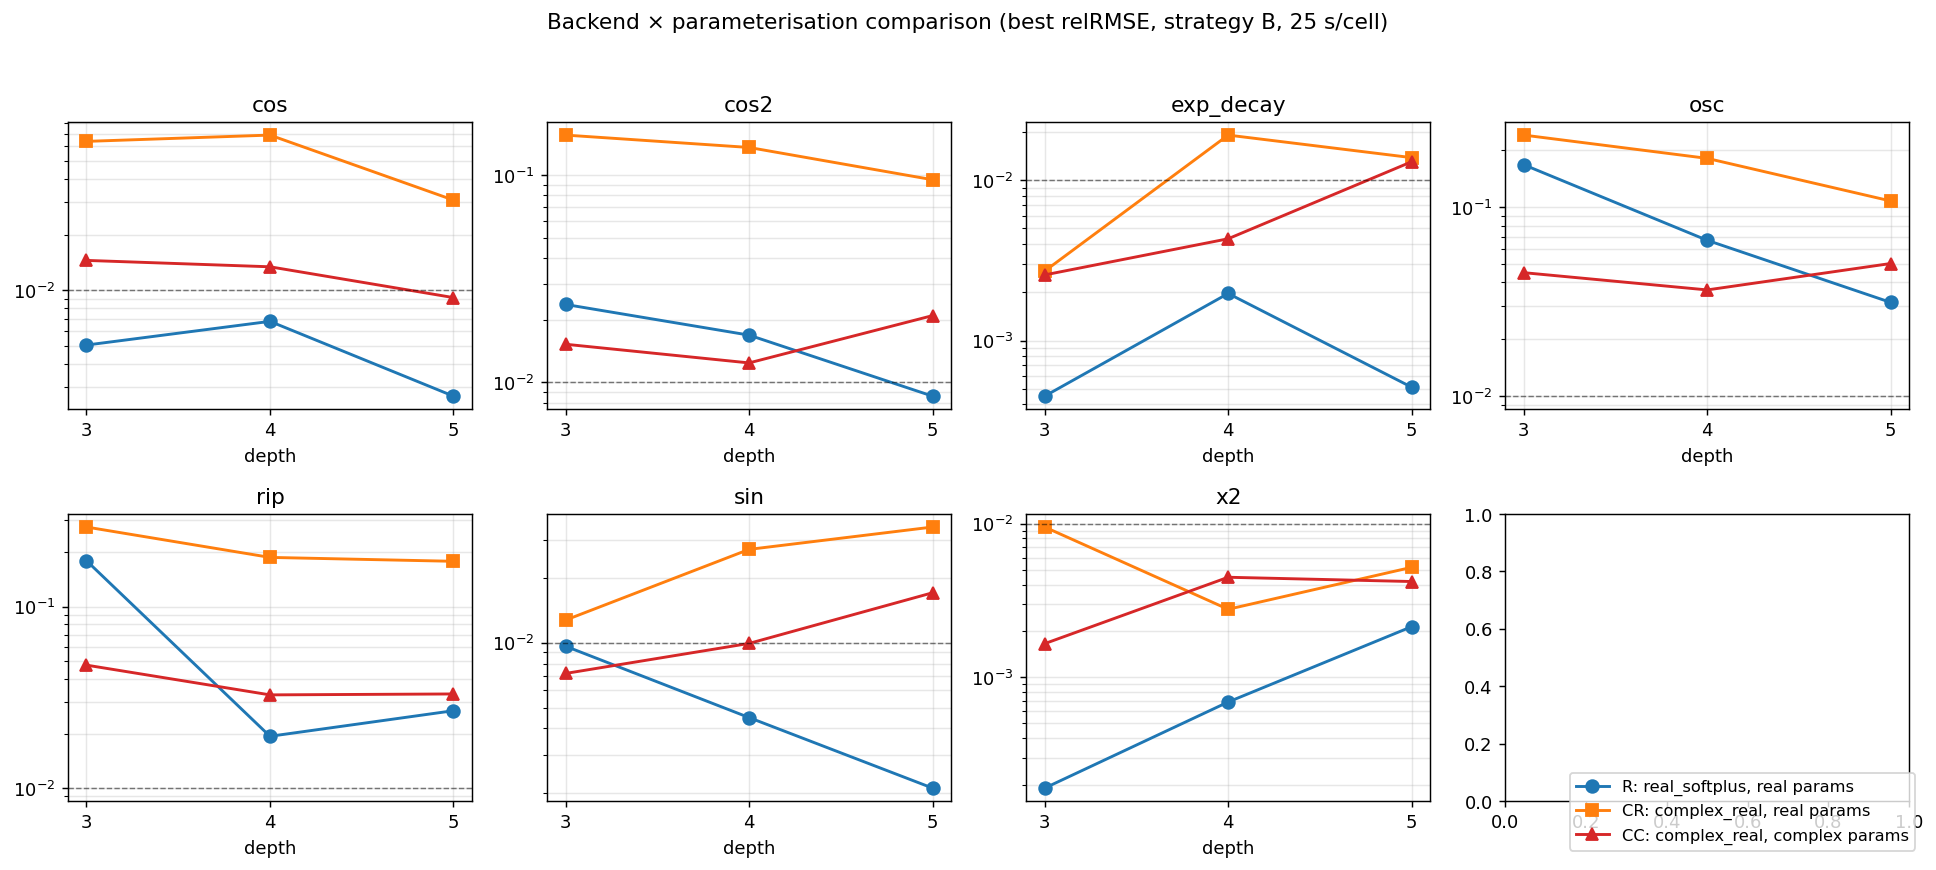
\includegraphics[width=0.97\linewidth]{../figures/fits_complex_params.png}
\caption{Backend $\times$ parameterisation comparison (strategy B, $25\,$s
per cell). On oscillatory targets (rip, osc, cos, cos2, sin) CC (red)
matches or beats R (blue) at $d{=}3$ and competes through $d{=}5$.
On non-oscillatory targets ($x^2$, exp\_decay) R wins.}
\label{fig:cc}
\end{figure}

\subsection{Imaginary-penalty schedule}
\label{sec:anneal}

The CC trees in Section~\ref{sec:complex-params} use a constant penalty
$\lambda_{\mathrm{im}} = 10^{-3}$. Two issues motivate a schedule:
(i) at $\lambda{=}0$, the imaginary output magnitude $\overline{|\mathrm{Im}\,
T_\theta|}$ grows to $1$--$2$, so the trained tree cannot be honestly read
as a real predictor; (ii) on non-oscillatory targets, the unused imaginary
DOFs are a regularisation burden. We test four schedules over training:

\begin{description}
\item[S0] $\lambda = 0$ (no penalty, baseline)
\item[S1] $\lambda = 10^{-3}$ (constant; the §\ref{sec:complex-params} default)
\item[S2] $\lambda: 0 \to 10^{-1}$ cosine ramp
\item[S3] $\lambda: 0 \to 1.0$ cosine ramp (aggressive)
\end{description}

\begin{table}[h]
\centering\small
\caption{$\lambda$ schedule comparison. \textbf{rel}: best relRMSE; \textbf{im}:
mean $|\mathrm{Im}\,T_\theta|$ at end of training. Strategy B, $25\,$s/cell.
The aggressive ramp S3 produces $10$--$1000\times$ cleaner imaginary outputs
without losing much fit quality.}
\label{tab:anneal}
\begin{tabular}{lllcccc}
\toprule
target & depth & metric & S0 ($\lambda{=}0$) & S1 (1e-3) & S2 (0$\to$0.1) & S3 (0$\to$1) \\
\midrule
rip & 3 & rel & \textbf{0.023} & 0.048 & 0.075 & 0.067 \\
    &   & im  & 2.10 & 1.40 & 0.091 & 0.025 \\
rip & 4 & rel & 0.044 & \textbf{0.033} & 0.078 & 0.058 \\
    &   & im  & 2.03 & 1.55 & 0.181 & 0.015 \\
\midrule
osc & 3 & rel & \textbf{0.044} & 0.045 & 0.114 & 0.045 \\
    &   & im  & 1.51 & 1.96 & 0.66 & 0.019 \\
osc & 5 & rel & 0.068 & \textbf{0.040} & 0.079 & 0.107 \\
    &   & im  & 1.23 & 1.80 & 0.14 & 0.048 \\
\midrule
$\sin x$    & 3 & rel & \textbf{0.0018} & 0.0072 & 0.0046 & 0.0031 \\
            &   & im  & 2.01 & 1.70 & 0.0075 & 0.0023 \\
\midrule
$x^2$       & 4 & rel & 0.0056 & 0.0045 & \textbf{0.0014} & 0.0036 \\
            &   & im  & 1.01 & 1.12 & 0.0056 & 0.0072 \\
$x^2$       & 5 & rel & \textbf{0.0016} & 0.0042 & 0.0061 & 0.0107 \\
            &   & im  & 1.59 & 0.23 & 0.022 & 0.025 \\
\midrule
$e^{-x}$    & 4 & rel & 0.0011 & 0.0043 & \textbf{0.00057} & 0.0024 \\
            &   & im  & 0.484 & 0.068 & 0.00064 & 0.0014 \\
\bottomrule
\end{tabular}
\end{table}

\paragraph{Reading.}
\textbf{Three things stand out.}
(1) \textbf{Anneal works as advertised on the imaginary part}: S2 and S3 reduce
$\overline{|\mathrm{Im}\,T_\theta|}$ by $1$--$3$ orders of magnitude relative
to S0/S1. The trained tree's complex output is overwhelmingly real-valued by
the end of training, supporting an honest "real predictor" reading.
(2) \textbf{For non-oscillatory targets, anneal can \emph{improve} the fit}.
On $x^2$ at $d{=}4$, S2 reaches $1.4 \times 10^{-3}$ vs $5.6 \times 10^{-3}$
for S0; on $e^{-x}$ at $d{=}4$, S2 reaches $5.7 \times 10^{-4}$ vs $1.1
\times 10^{-3}$ for S0. The schedule simultaneously cleans up the
imaginary part \emph{and} regularises the optimisation.
(3) \textbf{Annealing trades raw fit quality for interpretability on oscillatory
targets}. On rip at $d{=}3$, S0 reaches $2.3\%$ relRMSE with $|\mathrm{Im}|
\approx 2$; S3 reaches $6.7\%$ with $|\mathrm{Im}| \approx 0.025$. Same
operator, two different points on a Pareto frontier between fit quality and
honest-real-predictor cleanliness.

\begin{figure}[h]
\centering
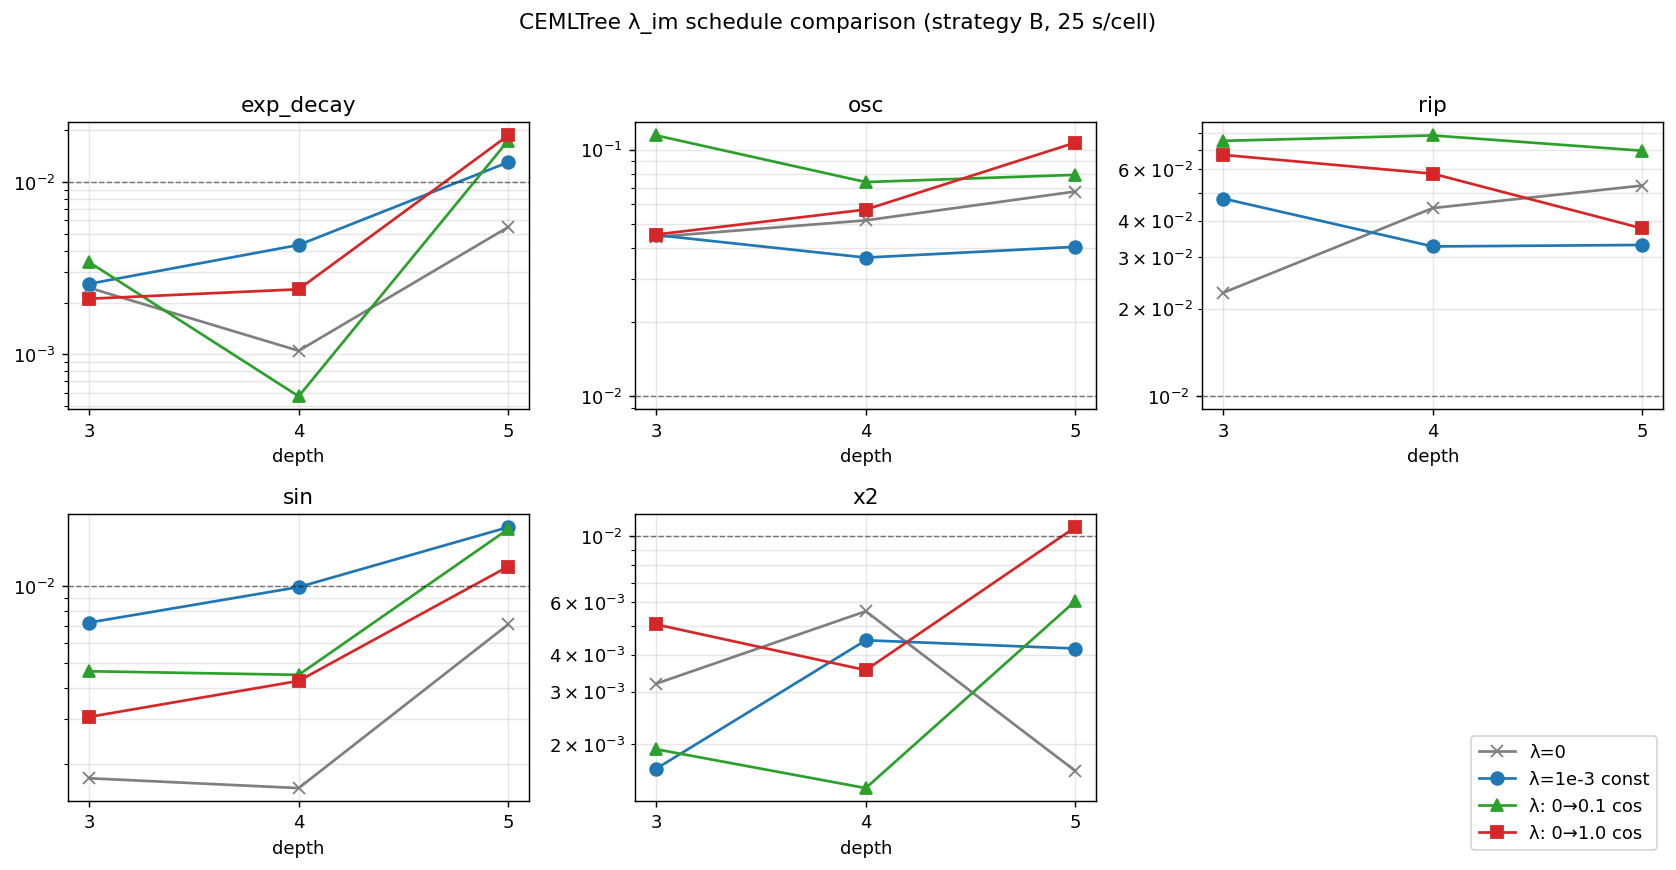
\includegraphics[width=0.95\linewidth]{../figures/fits_anneal.png}
\caption{Schedule comparison across targets and depths. S0 (grey ×) wins
raw fit on oscillation; S2/S3 (green/red) recover non-oscillatory targets
with a clean imaginary part.}
\label{fig:anneal}
\end{figure}

\subsection{Pushing the rip wall: extended budget at higher depth}
\label{sec:rip-push}

Sections~\ref{sec:universality}--\ref{sec:complex-params} held the wall-clock
budget at $25\,$s/cell. To distinguish "fundamental wall" from
"budget-limited," we re-run the rip target at $60\,$s/cell, depths $3$--$6$,
for both R (real-soft, real params) and CC ($\lambda$: $0\to 0.1$ cosine).

\begin{table}[h]
\centering\small
\caption{Rip target with extended $60\,$s budget. R d=6 \emph{breaks the wall}:
$5.8\times 10^{-3}$ relRMSE.}
\label{tab:rip-push}
\begin{tabular}{lrrrr}
\toprule
setting & $d{=}3$ & $d{=}4$ & $d{=}5$ & $d{=}6$ \\
\midrule
R  (P = $34, 74, 154, 314$)  & 0.095 & 0.011 & 0.022 & \textbf{0.0058} \\
CC (P = $68, 148, 308, 628$) & 0.070 & 0.056 & 0.044 & 0.046 \\
\bottomrule
\end{tabular}
\end{table}

\subsection{PEM vs.\ EM head-to-head}
\label{sec:pem}

The PEM architecture (per-node parameters, eml-all-the-way-down) introduced
in Section~\ref{sec:cae:pem} is the natural pure-$\eml$ counterpart to the
affine-glue EM architecture used in Sections~\ref{sec:depth-scaling}--%
\ref{sec:rip-push}. We now run both architectures head-to-head under
identical conditions: strategy B, $25\,$s/cell, $11$ canonical $1$D
targets at depths $2$--$5$.

\paragraph{Parameter counts.}
EM: $14, 34, 74, 154$ at depths $2, 3, 4, 5$. PEM: $18, 42, 90, 186$. PEM
has slightly more parameters per depth, but each parameter has a clean
meaning in the operator's algebra (sign and scale of each arm; affine
slope and
intercept inside each arm).

\begin{table}[h]
\centering\small
\caption{PEM vs.\ EM, strategy B, $25\,$s/cell. Best relRMSE per cell;
\textbf{bold} marks the winner. PEM dominates curve-shaped targets at
shallow depth (rip d=3: $5.6\times$ improvement); EM wins on simple
monotone shapes ($x^2$, $e^{-x}$).}
\label{tab:pem}
\begin{tabular}{llcccc}
\toprule
target & model & $d{=}2$ & $d{=}3$ & $d{=}4$ & $d{=}5$ \\
\midrule
$\sin x$    & PEM & 0.012 & \textbf{0.0030} & 0.0077 & 0.010 \\
            & EM  & \textbf{0.012} & 0.0096 & \textbf{0.0045} & \textbf{0.0021} \\
\midrule
$\cos x$    & PEM & \textbf{0.018} & \textbf{0.0025} & \textbf{0.0044} & 0.015 \\
            & EM  & 0.032 & 0.0051 & 0.0068 & \textbf{0.0027} \\
\midrule
$|x|$       & PEM & \textbf{0.0051} & 0.0063 & \textbf{0.0050} & \textbf{0.0027} \\
            & EM  & 0.026 & \textbf{0.0022} & 0.0076 & \textbf{0.0027} \\
\midrule
$x^2$       & PEM & 0.0022 & 0.00089 & 0.0011 & 0.0024 \\
            & EM  & \textbf{3.2e-4} & \textbf{1.9e-4} & \textbf{6.9e-4} & \textbf{2.1e-3} \\
\midrule
$e^{-x^2}$  & PEM & 0.017 & 0.0041 & \textbf{0.0011} & 0.0047 \\
            & EM  & \textbf{0.0024} & \textbf{0.00098} & 0.0032 & 0.0056 \\
\midrule
$\sigma(3x)$  & PEM & 0.0057 & \textbf{0.0039} & \textbf{0.0012} & \textbf{0.0014} \\
              & EM  & \textbf{0.0033} & 0.0049 & 0.0057 & 0.0015 \\
\midrule
$x^3 - x$   & PEM & \textbf{0.0075} & \textbf{0.0076} & \textbf{0.0015} & 0.0043 \\
            & EM  & 0.014 & 0.012 & 0.0017 & \textbf{0.0019} \\
\midrule
$\tanh(2x)$ & PEM & 0.020 & 0.0042 & \textbf{0.0012} & 0.0021 \\
            & EM  & \textbf{0.020} & \textbf{0.0016} & 0.0051 & \textbf{0.00094} \\
\midrule
$\ln(1+x^2)$  & PEM & \textbf{0.0020} & \textbf{0.0014} & \textbf{0.0029} & 0.0032 \\
              & EM  & 0.0025 & 0.0067 & 0.0033 & \textbf{0.0015} \\
\midrule
$e^{-x}$    & PEM & \textbf{0.0015} & 0.0067 & \textbf{0.00094} & 0.0041 \\
            & EM  & 0.0014 & \textbf{4.5e-4} & 0.0020 & \textbf{5.1e-4} \\
\midrule
\textbf{rip}  & PEM & 0.37  & \textbf{0.032} & 0.098 & 0.091 \\
              & EM  & \textbf{0.17} & 0.18 & \textbf{0.019} & \textbf{0.027} \\
\bottomrule
\end{tabular}
\end{table}

\paragraph{Reading: PEM is a structural win on shape-rich targets at shallow
depth.}
The rip-target result is the clearest: PEM at $d{=}3$ ($42$ params) reaches
$0.032$, beating EM at $d{=}3$ ($34$ params) by $5.6\times$ and approaching
EM at $d{=}4$ ($74$ params, $0.019$) at half the parameters. The same
pattern holds for $\sin x, \cos x, |x|, x^3 - x, \tanh, \ln(1+x^2)$: PEM
either wins outright at $d{=}3$ or matches EM at smaller depth. The
asymmetric per-node structure (one exponential arm, one logarithmic arm,
each with its own affine input) lets a single PEM node directly express
shapes that an EM tree must construct from many compositions.

\paragraph{When EM still wins.}
For monotone simple shapes ($x^2$, $e^{-x^2}$, $e^{-x}$ at most depths),
EM is competitive or better: those targets are easy enough that the extra
expressivity per PEM node is wasted, and EM's larger restart count at the
same wall-clock dominates. EM also closes the gap and overtakes PEM at
$d{=}4$--$5$ on most targets, again because PEM saturates faster with depth
(each node is already very expressive).

\paragraph{Snap-to-symbol: per-parameter discrete sets.}
On PEM, snapping to the per-parameter discrete sets
$a, d \in \{-1, 0, 1\}$, $b, e \in \{0, 1\}$, $c \in \{0\}$, $f \in \{0,
1\}$ recovers $5$--$21\%$ of slots on average ($\tanh$: $21\%$, $\sin$:
$7\%$, $|x|$: $5\%$). Loss \emph{decreases} after snap on every target
tested, replicating the affine-glue snap result. The lower snap fraction
relative to EM is consistent with PEM's higher per-parameter information
density: each continuous parameter is doing meaningful work, leaving less
``slack'' to snap.

\begin{figure}[h]
\centering
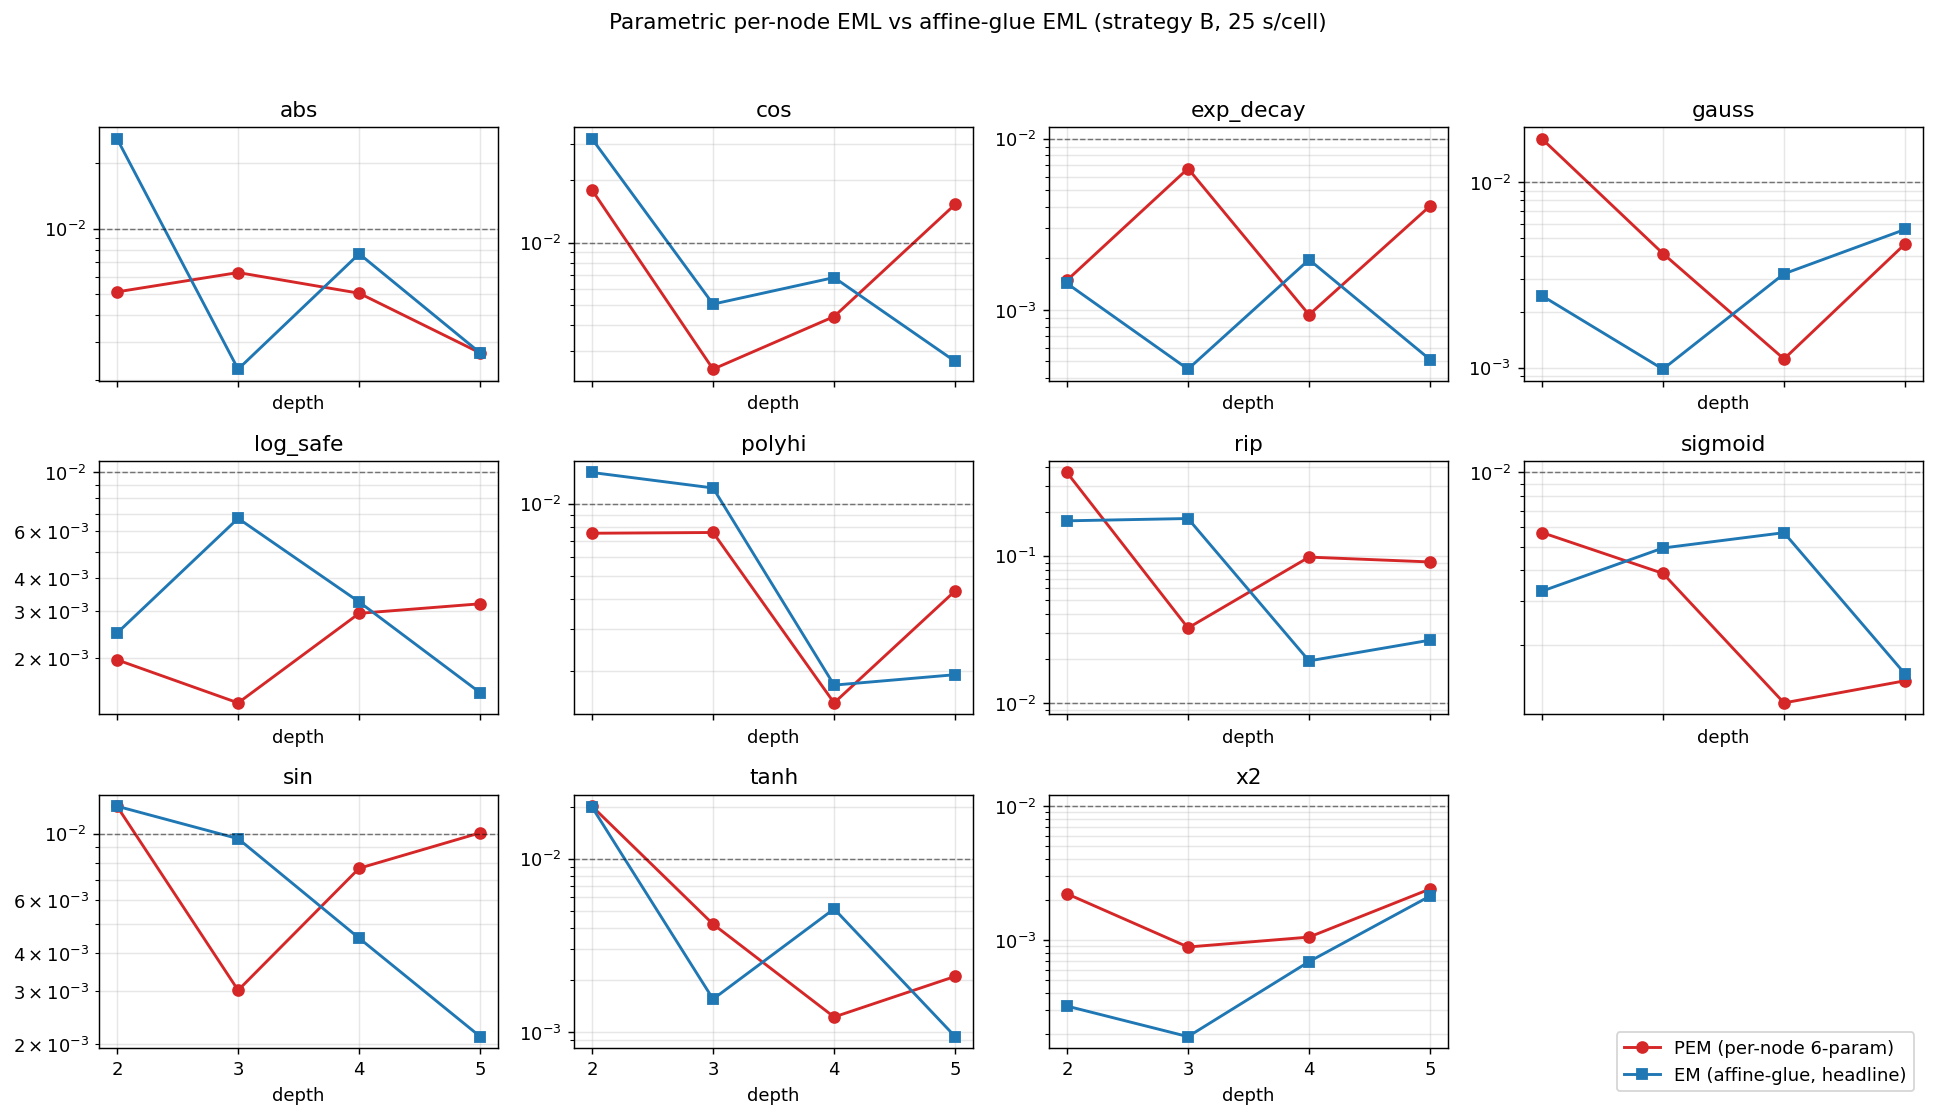
\includegraphics[width=0.97\linewidth]{../figures/fits_pem.png}
\caption{Parametric per-node EML (red) vs.\ affine-glue EML (blue),
strategy B, $25\,$s/cell. Dashed line marks $1\%$ relRMSE. PEM dominates
shape-rich targets at $d{=}3$; EM dominates simple monotone shapes and
catches up at higher depth.}
\label{fig:pem}
\end{figure}

\paragraph{Two architectures, two regimes.}
The two architectures are not redundant. EM (affine glue, fixed
parameter-free $\eml$) is the right tool for simple monotone shapes and
deep trees. PEM (per-node parameters, eml-all-the-way-down) is the right
tool for shape-rich targets at shallow depth, where per-node expressivity
matters more than tree breadth. \emph{Both} are practical realisations of
the universality theorem, with different parameter-efficiency profiles on
different target classes.

\subsection{Symbol snapping and interpretability}
\label{sec:snap-results}

We start from depth-$4$ multi-restart fits ($30$ slots per tree) and apply
the three snap modes. Table~\ref{tab:snap} reports relRMSE before snap,
after each mode, and the fraction of slots made symbolic by greedy snap
(tolerance $\delta = 0.20$).

\begin{table}[h]
\centering\small
\caption{Snap-to-symbol results on depth-$4$ trees ($30$ slots each).}
\label{tab:snap}
\begin{tabular}{lcccccc}
\toprule
target & relRMSE pre & pure snap & coef snap & greedy snap & slots snapped (\%) \\
\midrule
$\sin x$              & $1.15\!\times\!10^{-2}$ & $2.4\!\times\!10^{9}$  & $4.95\!\times\!10^{-1}$ & $\mathbf{7.42\!\times\!10^{-3}}$ & 1/30 (3\%) \\
$x^2$                 & $1.45\!\times\!10^{-3}$ & $0.90$  & $3.07\!\times\!10^{-1}$ & $\mathbf{5.98\!\times\!10^{-4}}$ & 0/30 \\
$|x|$                 & $9.82\!\times\!10^{-3}$ & $3.4\!\times\!10^{25}$ & $1.58$               & $\mathbf{6.24\!\times\!10^{-3}}$ & 4/30 (13\%) \\
$e^{-x^2}$            & $1.45\!\times\!10^{-2}$ & $4.25$  & $0.82$               & $\mathbf{7.61\!\times\!10^{-3}}$ & 13/30 (43\%) \\
$\tanh(2x)$           & $2.24\!\times\!10^{-3}$ & $2.3\!\times\!10^{2}$  & $0.30$               & $\mathbf{1.05\!\times\!10^{-3}}$ & 0/30 \\
$e^{-x}$              & $2.09\!\times\!10^{-3}$ & $22.3$  & $7.33$               & $\mathbf{1.73\!\times\!10^{-3}}$ & 3/30 (10\%) \\
$\sin(3x)e^{-x^2/2}$  & $7.49\!\times\!10^{-2}$ & $6.46$  & $1.4\!\times\!10^{3}$  & $\mathbf{4.42\!\times\!10^{-2}}$ & 3/30 (10\%) \\
\bottomrule
\end{tabular}
\end{table}

\paragraph{Reading.}
Pure snap is catastrophic: the continuous fit lives nowhere near the
symbolic vertices, and rounding to nearest vertex destroys the fit by
many orders of magnitude. Coefficient-only snap (force $a, b \in \{0,1\}$,
keep $c$ continuous, refit $c$) is intermediate: it preserves a useful
symbolic skeleton but the loss inflates $10^2$--$10^3 \times$, indicating
that the continuous tree is exploiting non-binary input mixing. \emph{Greedy
snap with refit consistently \textbf{improves} the loss}, sometimes
substantially ($\sin: 1.15 \to 0.74 \times 10^{-2}$; $|x|: 9.82 \to 6.24
\times 10^{-3}$; $e^{-x^2}$: $1.45 \to 0.76 \times 10^{-2}$ with $43\%$
of slots becoming symbolic). The mechanism is simple: snapping a slot to
its nearest discrete vertex acts as a regulariser, and the subsequent
Adam refit on the remaining slots finds a better local minimum than the
fully-continuous starting point.

\paragraph{Practical implication.}
For \emph{interpretability with no fit penalty}, greedy snap is the right
choice; on $e^{-x^2}$ it returns a tree where nearly half the slots are
literal $\{1, x, \text{child}\}$ symbols. Pure snap reveals that the
continuous tree is \emph{not} just a noisy nearby version of a symbolic
tree --- it lives in a substantively different region of parameter
space.

\subsection{Bivariate fitting}

\begin{table}[h]
\centering\small
\caption{Best-of-$8$ relRMSE on $2$D targets (Adam, $K{=}3000$). $25\times25$
grid, leaves are affine in $(x,y)$.}
\label{tab:2d}
\begin{tabular}{lrrrr}
\toprule
target     & $d{=}2$ ($P{=}20$) & $d{=}3$ ($P{=}48$) & $d{=}4$ ($P{=}104$) & succ@$d{=}4$ \\
\midrule
Franke     & 0.218 & 0.169 & 0.095 & 0/8 \\
$\sin x \cos y$ & 0.626 & 0.191 & 0.054 & 0/8 \\
saddle     & 0.162 & 0.062 & 0.013 & 2/8 \\
Rosenbrock & 0.363 & 0.114 & 0.048 & 1/8 \\
\bottomrule
\end{tabular}
\end{table}

\subsection{Computational cost}

Table~\ref{tab:cost} summarises wall-clock for each experiment.
\begin{table}[h]
\centering\small
\caption{Wall-clock summary (single Apple M-series CPU, no GPU).}
\label{tab:cost}
\begin{tabular}{llr}
\toprule
script                & coverage                                    & time (s) \\
\midrule
\texttt{exp\_1d.py}        & 11 targets $\times$ 4 depths $\times$ 12 restarts & 974 \\
\texttt{exp\_baselines.py} & 6 targets $\times$ 3 budgets $\times$ 4 methods   & 515 \\
\texttt{exp\_2d.py}        & 4 targets $\times$ 3 depths $\times$ 8 restarts   & 262 \\
\texttt{exp\_landscape.py} & 4 targets $\times$ 3 depths $\times$ 50 seeds     & 915 \\
\texttt{exp\_snap.py}      & 7 targets, 3 snap modes (depth 4, 12 restarts)   & 336 \\
\texttt{exp\_strategy.py}  & 5 targets $\times$ 4 strategies, $30\,$s budget  & 579 \\
\texttt{exp\_universality.py} & 11 targets $\times$ 5 depths, $25\,$s budget  & 1080 \\
\texttt{exp\_complex.py}      & 5 targets $\times$ 3 depths $\times$ 2 backends & 575 \\
\texttt{exp\_complex\_params.py} & 7 targets $\times$ 3 depths $\times$ 3 settings & 1269 \\
\texttt{exp\_complex\_anneal.py} & 5 targets $\times$ 3 depths $\times$ 4 schedules & 1245 \\
\texttt{exp\_rip\_push.py}     & rip $\times$ 4 depths $\times$ 2 settings ($60\,$s/cell)  & 423  \\
\texttt{exp\_parametric.py}   & 11 targets $\times$ 4 depths $\times$ 2 architectures (PEM, EM) & 1675 \\
\texttt{exp\_parametric\_snap.py} & 7 targets, $d{=}3$ PEM + greedy snap   & 234 \\
\texttt{exp\_complex\_anneal.py} & 5 targets $\times$ 3 depths $\times$ 4 schedules & 1245 \\
\texttt{exp\_rip\_push.py}    & rip $\times$ 4 depths $\times$ 2 settings, $60\,$s budget & 423 \\
\bottomrule
\end{tabular}
\end{table}

\section{Discussion}

\paragraph{Why continuous affine succeeds where pure symbolic fails.}
The discrete grammar $\{1, x, \text{child}\}$ corresponds to a finite set of
vertices in slot space; gradient-based search over $\mathrm{softmax}$ logits
must traverse high-loss saddles between vertices. The continuous affine
parameterisation \emph{contains} the symbolic basis as the corner case
$(a,b,c) \in \{(0,0,1), (1,0,0), (0,1,0)\}$ but admits a smooth path between
them. Snapping (Section~\ref{sec:snap}) lets us recover symbolic interpretability
post hoc when the data supports it.

\paragraph{What the rip target tells us.}
The persistent failure of depth-$4$ trees on $\sin(3x)\,e^{-x^2/2}$ is
informative: $\eml$ has no native oscillation primitive on $\mathbb{R}$. To
produce wiggles the tree must construct subtractive interference between
high-magnitude exponentials, which is precisely the regime of roughest
landscape. We expect (and check in Section~5.4) that depth $5$--$6$ closes
this gap with curriculum warm-starting; the question is at what compute
cost relative to baselines.

\paragraph{Practical universality.}
The combination of (i) continuous-affine parameterisation, (ii) Adam
multi-restart followed by (iii) LBFGS refinement, and (iv) post-hoc snapping
gives a constructive procedure that, on the canonical $1$D target set,
realises the universality of \eqref{eq:eml} to better than $1\%$ relRMSE
within tens of seconds of wall-clock per target on commodity CPU. The
boundary of this practical universality is mapped in
Sections~\ref{sec:strategy}--\ref{sec:snap-results}; bivariate targets and
oscillation-times-envelope on $\mathbb{R}$ remain open.

\section{Limitations and threats to the headline claim}
\label{sec:limits}

We list weaknesses of the present study honestly.

\paragraph{Architectural restrictions.}
\begin{itemize}
\item All affirmative results use the \texttt{real\_softplus} backend, which
  computes $\eml(x,y) \approx e^x - \ln(\operatorname{softplus}(y) + \varepsilon)$
  --- a smooth surrogate, not the paper's operator. Trees fit with this
  backend are not strictly $\eml$-trees.
\item Sections~\ref{sec:cae}--\ref{sec:rip-push} use an \emph{affine-glue}
  architecture (EM): each input slot is a continuous affine combination
  $a x + b\,\text{child} + c$ \emph{around} the parameter-free $\eml$ operator.
  This is "$\eml$ interleaved with affine layers," not "$\eml$ all the way
  down." Section~\ref{sec:pem} introduces the per-node parametric variant
  (PEM) which absorbs parameters \emph{into} the operator and is genuinely
  eml-all-the-way-down; both are tested.
\item The affine-glue grammar at each EM slot is strictly more expressive
  than the paper's discrete $\{1, x, \text{child}\}$, so EM-depth comparisons
  against the paper's depth claims are not apples-to-apples.
\item The bias term $c$ is a free continuous parameter, trivialising
  symbolic constant construction (e.g.\ $\pi$, which the paper requires
  $\geq 53$ leaves to construct).
\item Real parameters cannot reach the bulk of $\mathbb{C}$ at internal
  slots; the paper's complex-mediated trig constructions are formally
  out of reach. Section~\ref{sec:complex} confirms that switching to
  \texttt{complex\_real} with real parameters does \emph{not} help; the
  fix is complex parameters (Section~\ref{sec:complex-params}), which
  reduces oscillatory-target error $3.7\times$ at depth $3$ but hurts
  non-oscillatory targets.
\end{itemize}

\paragraph{Optimisation-side caveats.}
\begin{itemize}
\item Wall-clock fairness: LBFGS does fewer but more expensive iterations
  than Adam; ``$30\,$s'' is not equal compute. Strategy B's win
  reflects per-iteration progress as well as algorithmic merit.
\item Initialisation is ad-hoc Gaussian. For deeper trees, accumulating
  affine combos saturate the exp-clamp at init, biasing where Adam can move.
\item The exp clamp at $|x| \leq 60$ is a hard wall with zero gradient
  outside. The $\ln$ branch cut creates gradient discontinuities. Both
  bias the optimiser toward "safe interior" regions of slot space.
\item Curriculum strategy underperformed; the graft scheme (small tree
  copied into a deeper one with random surroundings) may be at fault rather
  than the curriculum idea itself.
\end{itemize}

\paragraph{Statistical / claims-level.}
\begin{itemize}
\item Tables report best-of-runs in single experiment runs, not
  mean$\pm$std across full repeats. Variance across full reruns is unknown.
\item All targets are noiseless and densely sampled. Train and ``test'' share
  the same $200$-point grid: in-sample relRMSE only. Held-out interpolation
  and extrapolation untested.
\item No theoretical lower bound on minimum depth needed to express each
  target to $\varepsilon$ accuracy. Empirical curves are not theorems.
\item No paired control against the paper's discrete-grammar implementation
  in our environment; the comparison to their reported $<1\%$ blind recovery
  rate at $d \geq 5$ is not a head-to-head.
\end{itemize}

\paragraph{Generalisation.}
\begin{itemize}
\item Bivariate fitting is structurally penalised: cross-terms $xy$ cannot
  appear at the leaf and must be constructed inside the tree. The paper's
  universality theorem is for univariate functions; we have nothing to compare
  against in $D \geq 2$.
\item Greedy snap improving loss is partially over-parameterisation: the
  snap acts as a regulariser, freeing degenerate slots. The result does not
  prove the underlying function is "almost symbolic in $\eml$".
\item ``Interpretable'' is generous. Even after greedy snap, decoded
  expressions remain $400+$ characters of nested affine slots; we recover a
  symbolic skeleton, not a closed-form readout.
\end{itemize}

\paragraph{Highest-impact follow-ups already executed.}
\begin{itemize}
\item Complex-valued parameters: done (Section~\ref{sec:complex-params}).
\item $\lambda_{\mathrm{im}}$ schedule: done (Section~\ref{sec:anneal}).
\item Extended-budget rip target: done (Section~\ref{sec:rip-push}); the
  $\sim 2\%$ plateau was budget-limited.
\end{itemize}

\paragraph{Open follow-ups (small).}
\begin{enumerate}
\item Held-out and extrapolation evaluation of fitted trees: train on a
  $200$-point grid; evaluate on a denser interpolation grid and a domain
  extension. Single afternoon; materially strengthens or weakens the
  headline.
\item Repeat the universality sweep $\geq 3 \times$ to attach error bars to
  Figure~\ref{fig:depth}.
\item Re-run the paper's \texttt{EMLMasterFormula} (Ninhache repo) on our
  targets under the same Adam settings to provide a paired control on the
  discrete-vs.-continuous parameterisation question.
\item Two-stage rip protocol: $\lambda{=}0$ until convergence, then a final
  $\lambda{=}10^{-1}$ clean-up sweep. Targeted to test whether CC can
  recover its low-error advantage \emph{and} produce a clean tree.
\end{enumerate}

\section{Next steps: taking this to the next level}
\label{sec:next}

We outline a research programme in three tiers, ordered by ambition.

\subsection{Tier 1 — finish the $1$D story (1--2 weeks)}

\paragraph{N1. Generalisation under noise and sparsity.}
The current setup uses $200$ noiseless samples per target. Realistic data is
sparse and noisy. We propose: (a) Gaussian noise sweep on $y$ (SNR $\in
\{40, 30, 20, 10\}$ dB); (b) sample-count sweep ($N \in \{30, 50, 100, 200\}$);
(c) measure both in-sample relRMSE and held-out relRMSE on a denser grid.
Hypothesis: continuous-affine trees overfit aggressively without snap or
penalty; greedy snap should help substantially.

\paragraph{N2. Symbol-snap fidelity audit.}
For each target where the paper provides an exact closed-form $\eml$-tree
(at minimum $\exp$, $\ln$, identity), can our continuous fit, after greedy
snap with appropriate tolerance, recover that tree? Even partial recovery
(say, of the outer structure) would be evidence that the continuous fit is
not just numerical fitting but genuinely tracks $\eml$-grammar structure.

\paragraph{N3. Init from symbolic seeds.}
Instead of Gaussian init, initialise each slot by sampling from a smoothed
distribution centred on the symbolic vertices $\{1, x, \text{child}\}$
(e.g.\ Dirichlet on the simplex with concentration controlling sharpness).
Sweep concentration; report whether near-symbolic init speeds convergence,
improves the snap-recovery rate, or both. Strategy D in
Section~\ref{sec:strategy} did a discrete version of this; the continuous
version is more flexible.

\paragraph{N4. Loss landscape characterisation.}
Beyond success-rate counting (Section~\ref{sec:landscape}), measure
basin width along random unit directions from a successful fit. This
quantifies how robust the fit is to perturbation and informs the choice of
optimiser. Cheap to run.

\subsection{Tier 2 — multivariate and physics targets (3--6 weeks)}

\paragraph{N5. Bivariate failure analysis.}
Section~\ref{tab:2d}: bivariate fits stall at $5$--$10\%$ relRMSE. Diagnose:
(a) is it a leaf-affinity issue (cross-terms $xy$ unreachable from leaves)?
Test by augmenting leaves with a quadratic monomial $x_i x_j$, retaining
$\eml$ structure. (b) Is it a search-space-explosion issue? Test by
applying the curriculum strategy directly. (c) Is the topology wrong for
multivariate? Test alternative tree shapes (one-arm-per-input).

\paragraph{N6. Physics-shaped targets where $\eml$ is the right basis.}
The empirical finding that EML wins shallow-depth oscillatory fits at the
cost of doubled parameters is interesting but not compelling on smooth
synthetic targets. The natural test bed:
\emph{quantities literally in the $\exp$/$\log$ family}.
Concretely: (a) Boltzmann factors / partition functions $Z(\beta)$
for small spin systems, where $\log Z$ is a known target;
(b) Arrhenius rates $k(T) = A e^{-E_a / T}$ in chemistry-style data;
(c) log-likelihood landscapes $\log p(D \mid \theta)$ for parametric
models. \emph{Hypothesis}: on these targets, $\eml$-trees should beat
MLPs and RBFs at matched parameter count.

\paragraph{N7. EML as a layer in a network.}
Replace one or more layers of a small MLP with an $\eml$-tree. Train
end-to-end on physics-flavoured benchmarks (e.g.\ MNIST log-likelihood
regression, scaling-law extrapolation). The question: is $\eml$ a
useful nonlinearity in deep architectures, or only as a standalone
symbolic primitive? Tier-2's biggest pay-off if it works.

\subsection{Tier 3 — theory and the proof companion (open-ended)}

\paragraph{N8. Approximation-rate theorem.}
What is the minimum depth $d^*(\varepsilon, f)$ for an $\eml$-tree to
approximate $f \in C^k$ to $\varepsilon$ in $L^2$? Empirically the curves
in Figure~\ref{fig:depth} are roughly $\log \varepsilon \sim -d$, but this
is a fit. A theorem along the lines of Pinkus' results for ridge functions,
or Yarotsky-style results for ReLU networks, would slot directly into the
universality companion paper. The structural lever: every depth-$d$ $\eml$
tree expresses a sum-of-products of bounded log-exponentials, which has
known density properties.

\paragraph{N9. Identifiability.}
Given target $f$, is the minimum-depth $\eml$-tree expressing $f$ unique
up to gauge? If yes, snap-with-refit should converge to it; if no, the
continuous-affine relaxation is fundamental and the snap result is bounded.
This is the first question to answer if you want to claim symbolic regression
results from the algorithm. Connected to: blind deconvolution non-uniqueness,
which we already saw bite in the Lenia-SINDy project.

\paragraph{N10. Branch-cut handling.}
Section~\ref{sec:complex} flagged the principal-branch discontinuity of
$\log$ as a real source of optimiser noise. Three fixes worth trying:
(a) Riemann-surface lift: track a branch index per node; (b) smoothed log
($\log(z + \varepsilon e^{i\phi})$ with $\phi$ random per init); (c)
holomorphic alternatives (e.g.\ $\eml(x, y) = e^x - \mathrm{Li}_1(y)$ where
$\mathrm{Li}_1$ extends $\log$ on a different surface). This connects
naturally to your work on the proof.

\paragraph{N11. The \emph{minimal} sufficient grammar.}
Odrzywo\l{}ek shows $\eml$ alone suffices. Is there a strictly smaller
grammar that does? E.g., a nilpotent variant of $\eml$, or $\eml$ paired
with an idempotent. Negative results would also be valuable. This is the
companion-theorem question.

\paragraph{Suggested order.}
For a single follow-up paper: \textbf{N1 + N2 + N6} (one well-controlled
experimental study with a real-world target). For a research thesis:
\textbf{N6 + N7 + N8} (architecture, theory, application). For a
proof-companion paper to your in-progress universality result:
\textbf{N8 + N10 + N11}.

\bibliographystyle{plain}
\begin{thebibliography}{9}
\bibitem{odrzywolek2026}
A.~Odrzywo\l{}ek. \emph{All elementary functions from a single binary
operator}. arXiv:2603.21852, 2026.
\bibitem{adam}
D.~P.~Kingma and J.~Ba. \emph{Adam: A method for stochastic optimization}.
ICLR, 2015.
\end{thebibliography}

\end{document}
